En esta sección se analiza empíricamente el comportamiento de Fuerza Bruta, Programación Dinámica (DP) y los
dos enfoques Greedy: el primero basado en priorizar capítulos que brinden la mayor satisfacción neta
 (\texttt{Greedy(v)}) y el segundo basado en el mayor ratio de satisfacción por minuto invertido (\texttt{Greedy(v/t)}).

\subsection*{Calidad de las Soluciones Heurísticas}

Al tomar a DP como el $100\%$ de optimalidad (dado que siempre halla la solución optima), se logra medir el grado de éxito
de las alternativas Greedy en casos de diferente magnitud. Tal como lo muestra la Figura~\ref{fig:calidad_porcentaje},
si bien su desempeño es subóptimo, es consistentemente decente considerando el nulo coste de recursos y su eficiencia 
temporal. \texttt{Greedy(v)} ronda un porcentaje de acierto cercano al $71.7\%$ en promedio, levemente superior al $69.1\%$ 
promedio de \texttt{Greedy(v/t)}, lo que sorprende, ya que se esperaria que al considerar el tiempo en le ecuación su valor
de optimalidad fuera mejor. 

\begin{figure}[H]
    \centering
    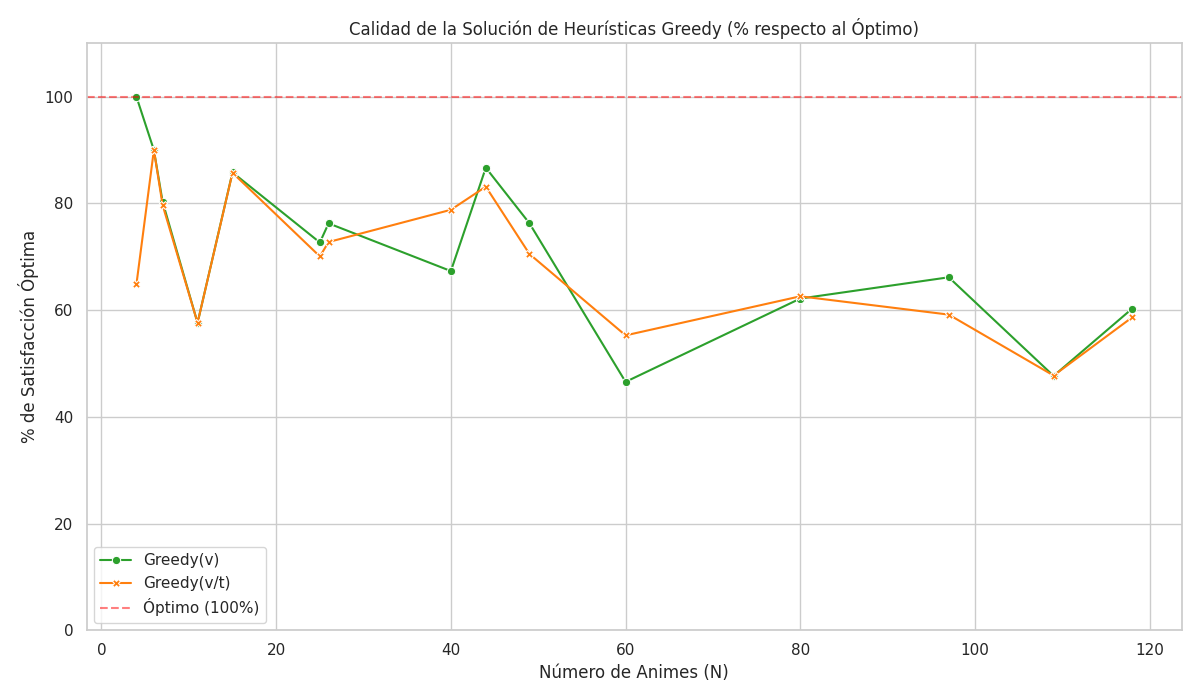
\includegraphics[width=0.7\textwidth]{IMG/comparativa_calidad_porcentaje.png}
    \caption{Porcentaje de optimalidad alcanzado por las heurísticas Greedy en distintas instancias (DP representa la línea base del $100\%$).}
    \label{fig:calidad_porcentaje}
\end{figure}

Llama la atención las caídas drásticas de calidad que sufre el algoritmo.(por ejemplo, descendiendo debajo del $60\%$ en
 casi todo los test luego de superar los $60$ animes). Esto puede ocurrir debido a la naturaleza del algoritmo que prioriza
apresuradamente decisiones egoístas que consumen tempranamente el tiempo o la energía en animes que dan beneficios inmediatos,
impidiendo explorar combinaciones que en un enfoque global (como DP) traerian un mayor beneficio.

\subsection*{Comportamiento de la Memoria}

El uso aislado de la memoria mediante \texttt{fork} permitió obtener la Figura~\ref{fig:comparativa_memoria}, en la cual es
evidente el \textit{trade-off} que efectúa DP para obtener su solucion optima. Mientras los algoritmos Greedy se mantienen
lineales e inalterados alrededor de $2000$ KB sin importar el tamaño del dataset, DP dispara su consumo drásticamente. Su
tabla de estados multidimensional exige de espacio en función directa a $M \cdot E \cdot N$, llegando a requerir más de 
$24000$ KB (un aumento superior al $1000\%$) para problemas grandes. Por su lado, la Fuerza Bruta mantiene un uso de memoria
extremadamente bajo, pues solo almacena el stack de llamadas recursivas.

\begin{figure}[H]
    \centering
    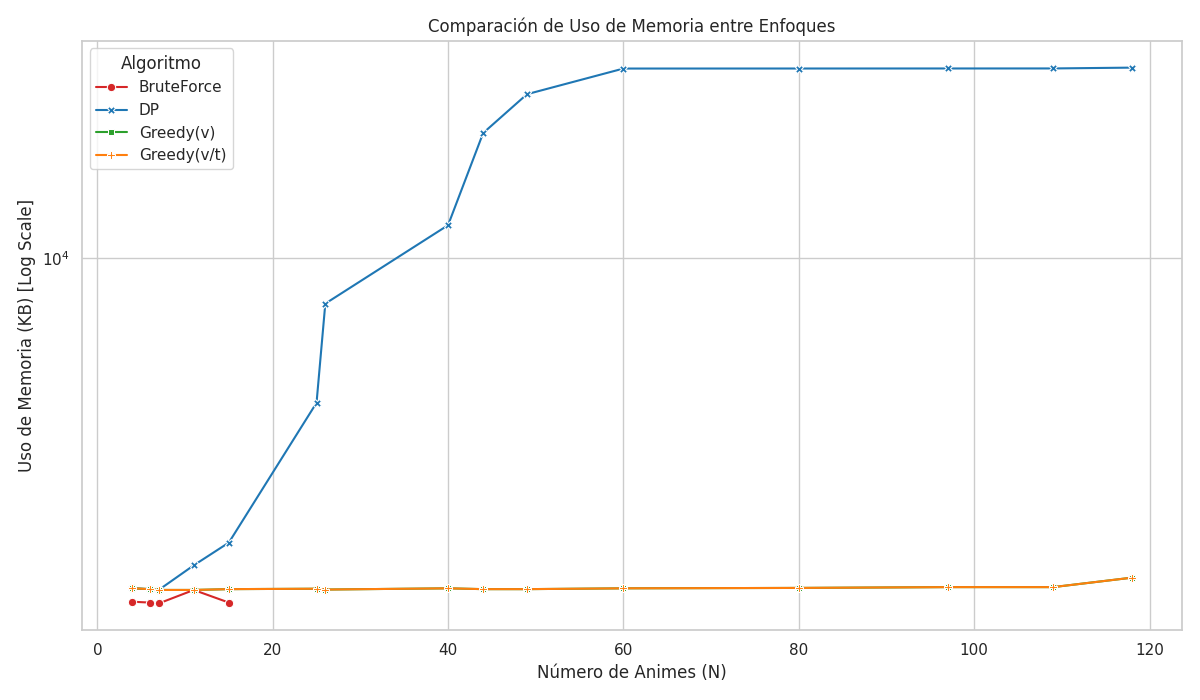
\includegraphics[width=0.7\textwidth]{IMG/comparativa_memoria.png}
    \caption{Comparativa de la memoria máxima en KB consumida por algoritmo.}
    \label{fig:comparativa_memoria}
\end{figure}

\subsection*{Análisis Temporal y Parámetros de Dispersión}

Aqui es donde destaca bastante el comportamiento que tiene el enfoque de Fuerza Bruta, ya que su debilidad no es su memoria, 
sino su exponencialidad temporal. Según los datos, incluso al usar dataset de $N=11$ a $N=15$, su tiempo se dispara un 
$\sim 2350\%$ (de $1.5$ a $36.5$ ms), descartándose de inmediato para casos serios.

\begin{figure}[H]
    \centering
    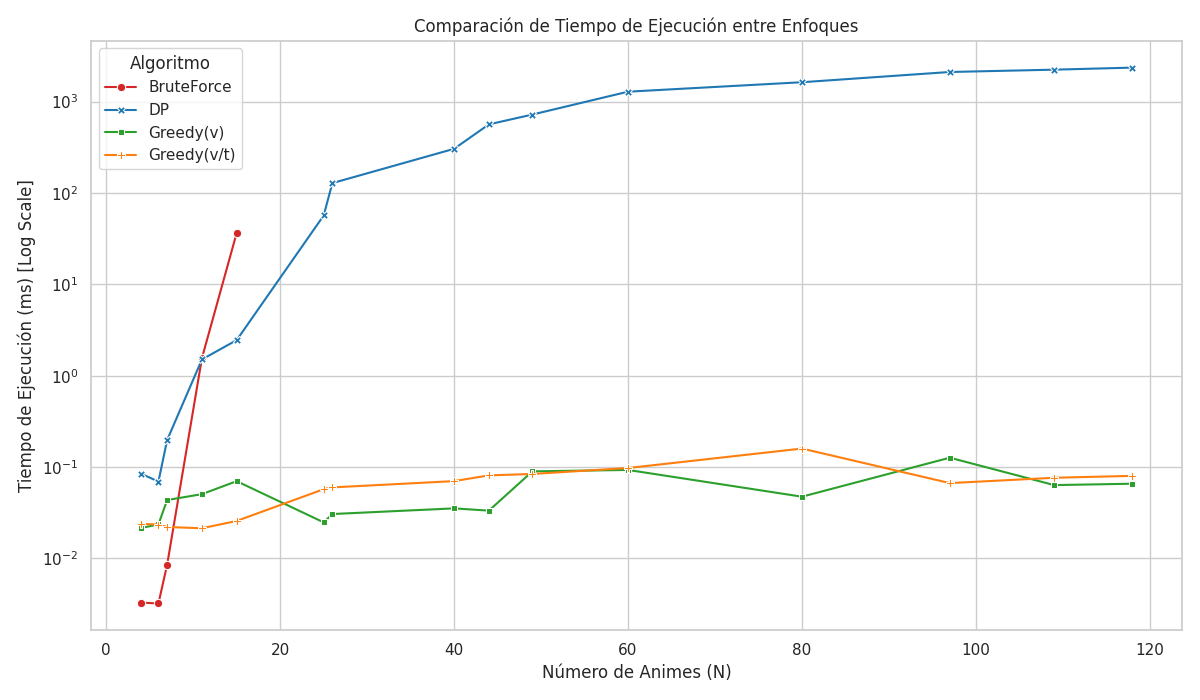
\includegraphics[width=0.7\textwidth]{IMG/comparativa_tiempos.png}
    \caption{Escalabilidad de los tiempos de ejecución.}
    \label{fig:comparativa_tiempos}
\end{figure}

El enfrentamiento real ocurre entre DP y los Greedys. Como muestra la Figura~\ref{fig:comparativa_tiempos}, DP se muestra enormemente
superado en terminos de velocidad en comparacion, demandando una cantidad para nada descartable de tiempo para instancias grandes, en contraste con
los algoritmos Greedy que convergen en menos de un milisegundo ($< 0.1$ ms) sin inmutarse mayormente. Este es el sacrificio estricto
de DP, y es que sufre de ser varias órdenes de magnitud más lento a cambio de la respuesta óptima asegurada.

\begin{figure}[H]
    \centering
    \begin{minipage}{0.48\textwidth}
        \centering
        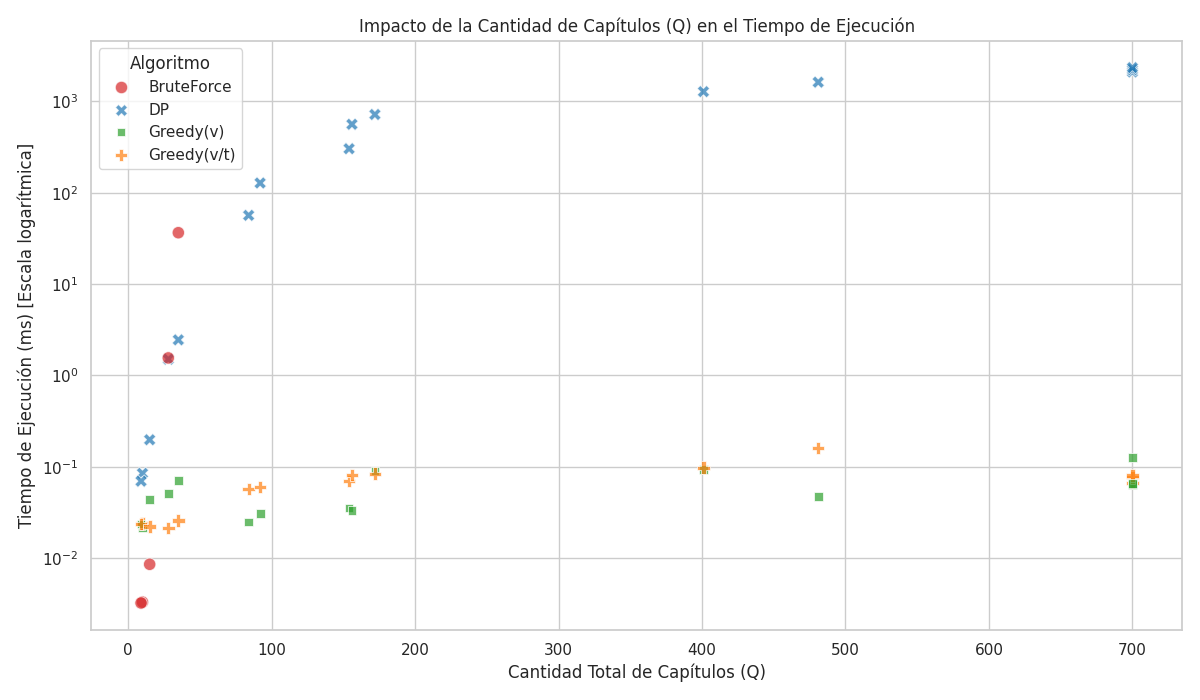
\includegraphics[width=\linewidth]{IMG/Dispersión_tiempo_vs_Cantidad_total_de_capitulos.png}
        \caption{Dispersión de Tiempo vs Capítulos. DP se desvía ascendentemente al aumentar $Q$.}
        \label{fig:disp_tiempo}
    \end{minipage}\hfill
    \begin{minipage}{0.48\textwidth}
        \centering
        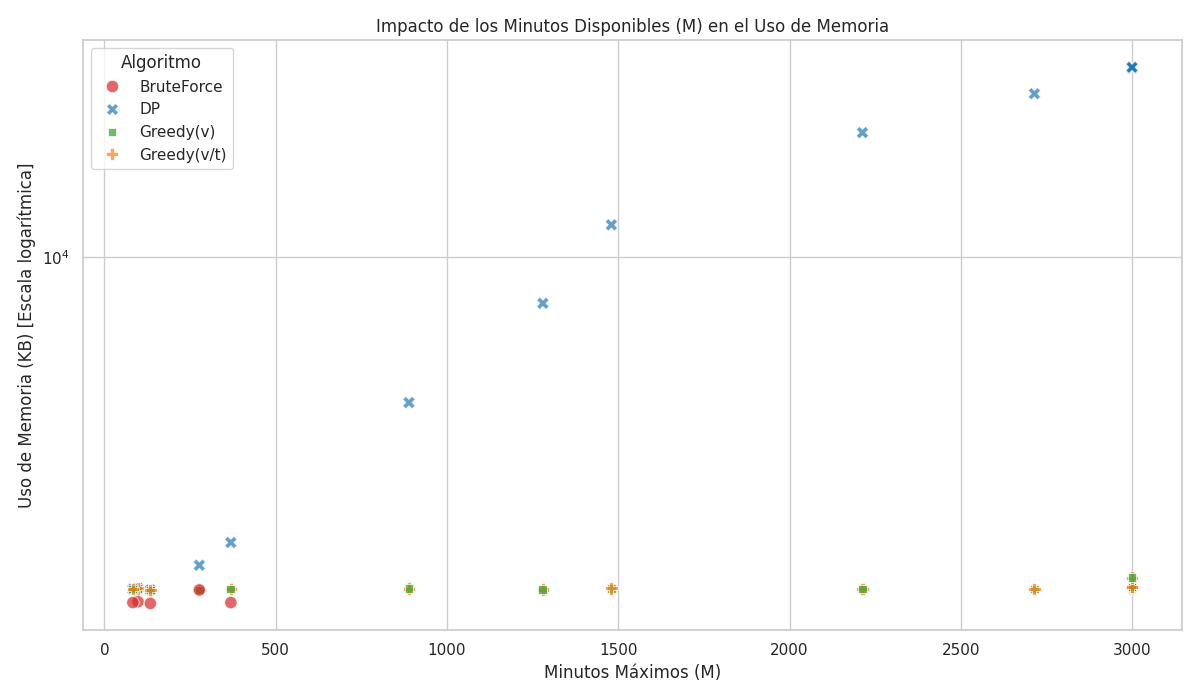
\includegraphics[width=\linewidth]{IMG/Dispersión_memoria_vs_Minutos_disponibles.png}
        \caption{Dispersión Memoria vs Minutos. Muestra la directa correlación lineal con el límite $M$ para DP.}
        \label{fig:disp_mem}
    \end{minipage}
\end{figure}

Por último, los gráficos de dispersión (Figuras~\ref{fig:disp_tiempo} y~\ref{fig:disp_mem}) refuerzan la complejidad de DP.
El consumo de recursos crece descontroladamente al aumentar los minutos disponibles $M$ (o la energía $E$), porque su espacio
 de estados se amplifica de forma multiplicativa. Los algoritmos Greedy resultan ser inmunes al aumento de $M$ y $E$, viéndose
afectados únicamente por la cantidad total de capítulos $Q$ al momento de realizar los ordenamientos.
